% !TEX TS-program = lualatex
% !BIB TS-program = biber
%\documentclass[handout]{beamer}
\documentclass{beamer}
\input{../common/misomva}
\newcommand{\misoclasstinytitleslide}{Partially based on material by:  Mikhail Belkin, \\[-1em] 
Jerry Zhu, Olivier Chapelle, Branislav Kveton}
\newcommand{\misoclassdate}{}
\begin{document}
% Topic-specific title slide
\newcommand{\topictitle}{Laplacian SVMs and Max-Margin Graph Cuts}
\newcommand{\topicsubtitle}{Inductive SSL Methods}
\renewcommand{\misoclasstinytitleslide}{Partially based on material by:  Mikhail Belkin, Partha Niyogi, \\[-1em] Olivier Chapelle, Bernhard Sch\"olkopf}

\MakeTopicSlide

\begin{frame}
\frametitle{SSL with Graphs: Laplacian SVMs}
\[
f^\star = \argmin_{f \in \cH_\cK}  \sum_i^{n_l} \mcolA{\max\left(0,1-yf\left(\bx\right)\right)} 
+ \gamma_1 \mcolB{ \|f\|^2_\cK }
+ \gamma_2 \mcolB{ \bff\transpose\bL\bff }
\]
$\cH_\cK$ is nice and expressive. \\ \smallskip
\pause
\vspace{-0.5em}
\begin{flushright}
\questionbox{Can there be a problem with certain $\cH_\cK$?}                                                            \end{flushright}
\pause
\vspace{-0.5em}
We look for $f$ only in $\cH_\cK$. \\ \smallskip
\pause
If it is simple (e.g., \textbf{linear})  minimization of $\bff\transpose\bL\bff$ can perform badly. 
\pause
\begin{center}
Consider again this 2D data and linear $\cK$.
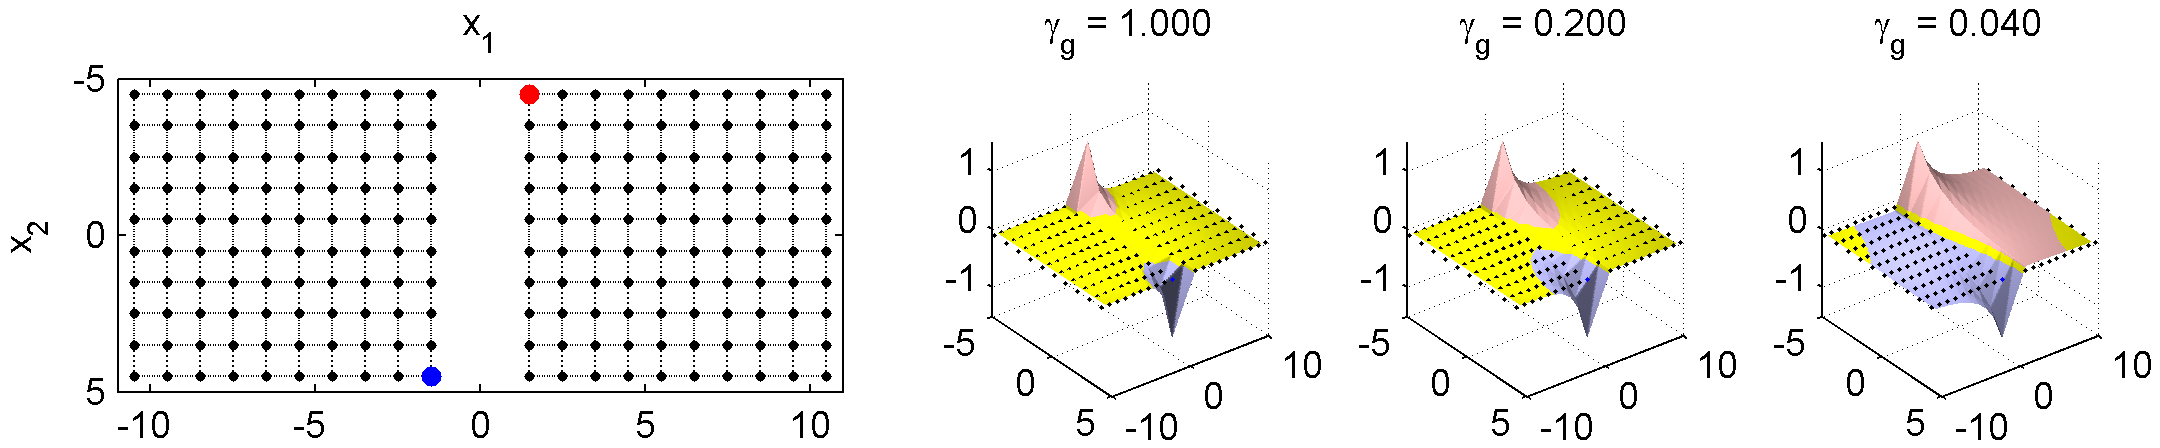
\includegraphics[width=\columnwidth]{../img/HFS}                                                      \end{center}
\end{frame}



%%%%%%%%%%%%%%%%%%%%%%%%%%%%%%%%%%%%%%%%%%%%%%%%%%%%%%%%%%%%
\begin{frame}
\frametitle{SSL with Graphs: Laplacian SVMs}

Linear $\cK \equiv$ 
\pause
functions with slope $\alpha_1$
and intercept $\alpha_2$.
\pause
\begin{equation*}
  \min_{\alert{\alpha_1, \alpha_2}} 
  \sum_{i}^{n_l} \mcolA{V(f, \bx_i, y_i)} +
  \mcolB{\gamma_1 \pause \left[\alpha_1^2 + \alpha_2^2\right] +
  \gamma_2 \bff\transpose \bL \bff}  
\end{equation*}
\pause
For this simple case we can write 
down $\bff\transpose \bL \bff$ explicitly. \\ \smallskip
\pause
\vspace{-1em}
\begin{align*}
  \action<+->{\mcolB{\bff \transpose \bL \bff}}
  \ \action<+->{= & \ \ \frac{1}{2} \sum_{i, j} w_{ij} (f(\bx_i) - f(\bx_j))^2}
  \nonumber \\
  \ \action<+->{= & \ \ \frac{1}{2} \sum_{i, j} w_{ij}
  (\alpha_1 (\bx_{i1} - \bx_{j1}) + \alpha_2 (\bx_{i2} - \bx_{j2}))^2}
  \nonumber \\
  \ \action<+->{= & \ \ \frac{\alpha_1^2}{2} \underbrace{\sum_{i, j} w_{ij}
  (\bx_{i1} - \bx_{j1})^2}_{\Delta = 218.351} +  \frac{\alpha_2^2}{2} \underbrace{\sum_{i, j} w_{ij}
  (\bx_{i2} - \bx_{j2})^2}_{\Delta = 218.351}}
%   \label{eq:linear manifold}
\end{align*}


\end{frame}
%%%%%%%%%%%%%%%%%%%%%%%%%%%%%%%%%%%%%%%%%%%%%%%%%%%%%%%%%%%%
\begin{frame}
\frametitle{SSL with Graphs: Laplacian SVMs}

2D data and linear $\cK$ objective

\begin{align*}%[Linear support vector machine]
  \min_{\alpha_1, \alpha_2} \ 
\sum_{i}^{n_l} \mcolA{V(f, \bx_i, y_i)} +
  \mcolB{\left(\gamma_1 + \frac{\gamma_2 \Delta}{2}\right)
  [\alpha_1^2 + \alpha_2^2]}
\end{align*}
\pause
Setting $\overline{\gamma} = \left(\gamma_1 + \frac{\gamma_2 \Delta}{2}\right)$: \pause
\begin{align*}
	\min_{\alpha_1, \alpha_2}  
\sum_{i}^{n_l} \mcolA{V(f, \bx_i, y_i)} +
  \mcolB{\overline{\gamma}[\alpha_1^2 + \alpha_2^2]}
%   \label{eq:linear SVM}
\end{align*}
\pause 
\questionbox{What does this objective function correspond to?}
\pause 
\onslide<handout:0>{\notecol{%
Linear SVM}} 
\moveb
\pause
The only influence of unlabeled data is through $\overline{\gamma}$.
\pause
\begin{flushright}
The same value of the objective as for supervised learning
for some $\gamma$ \textbf{without the unlabeled data}!
\notecol{This is not good.}
\end{flushright}
\end{frame}
%%%%%%%%%%%%%%%%%%%%%%%%%%%%%%%%%%%%%%%%%%%%%%%%%%%%%%%%%%%%
\begin{frame}
\frametitle{SSL with Graphs: Laplacian SVMs}

\begin{center}
LSVM for 2D data and linear $\cK$ only changes the slope \\ \bigskip
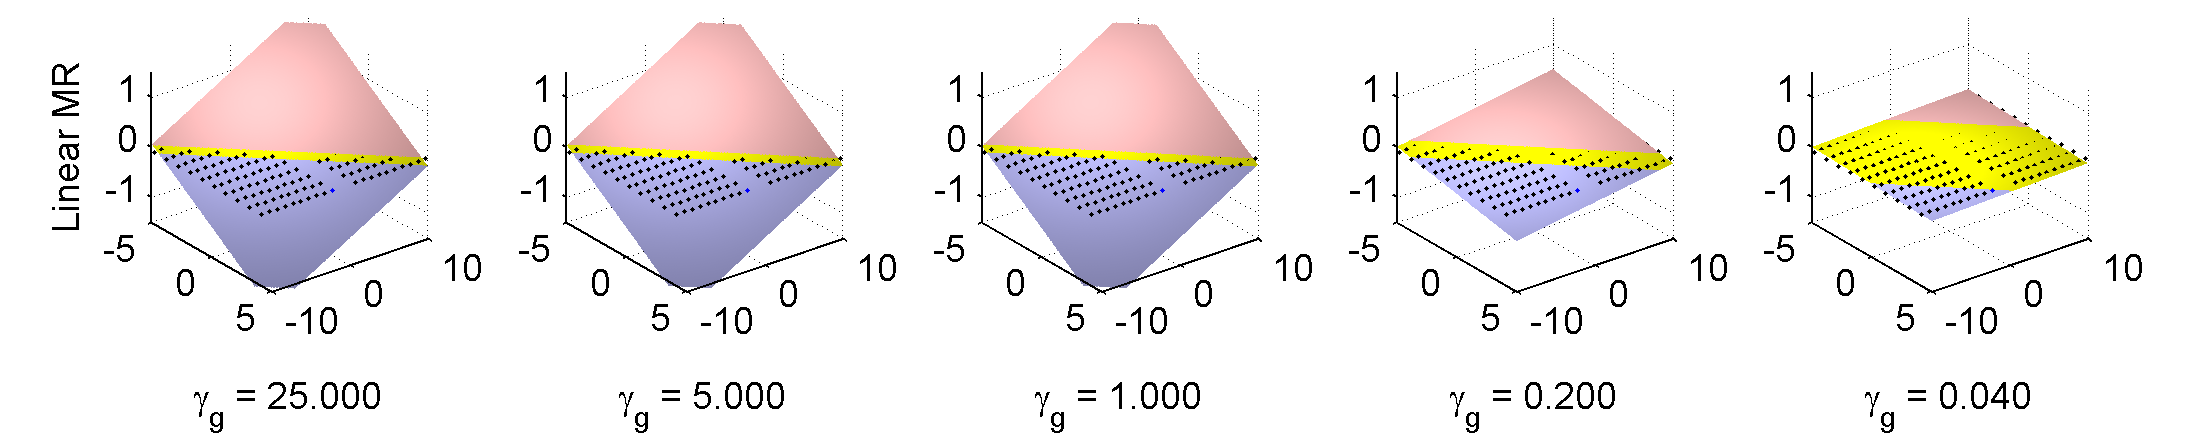
\includegraphics[width=\columnwidth]{../img/SyntheticCuts1b}
\pause
\questionbox{What would we like to see?}\\ \bigskip
\pause
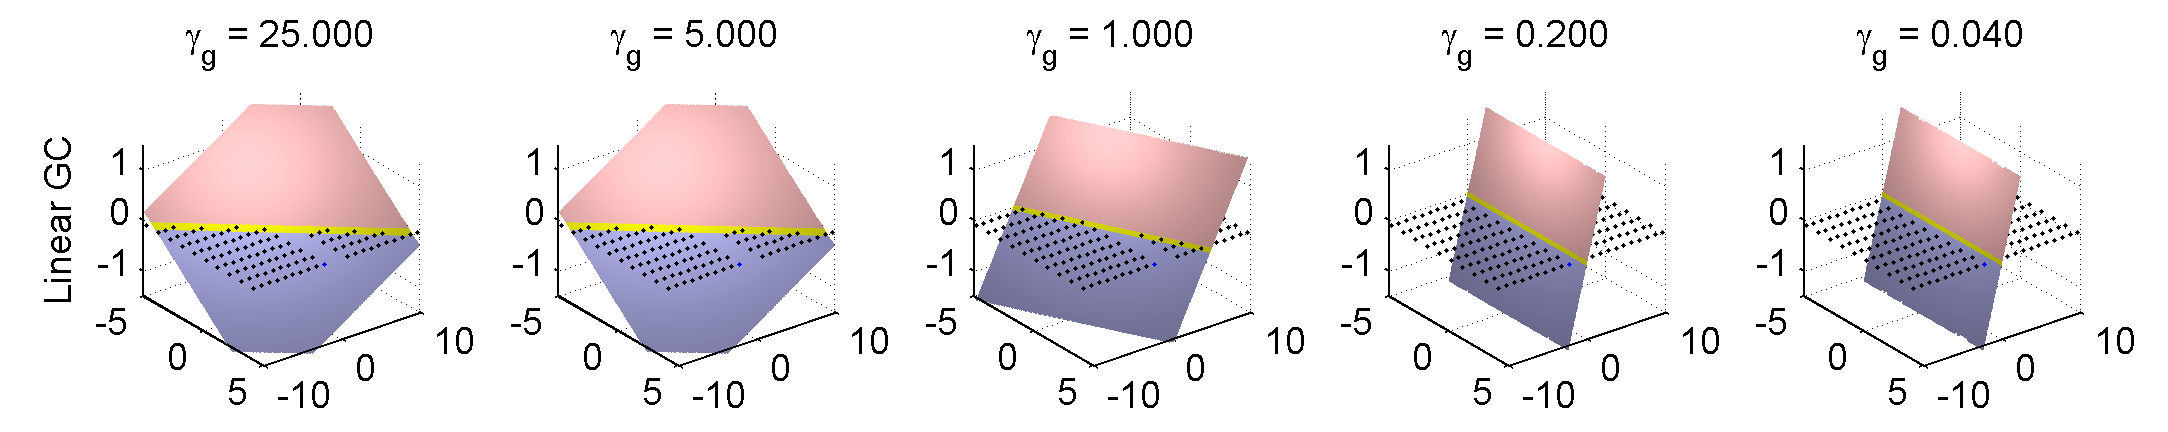
\includegraphics[width=\columnwidth]{../img/SyntheticCuts1a}
\pause
\yellbox{One solution: We use the unlabeled data \textbf{before} optimizing over $\cH_\cK$!}
\end{center}
\end{frame}
%%%%%%%%%%%%%%%%%%%%%%%%%%%%%%%%%%%%%%%%%%%%%%%%%%%%%%%%%%%%
\begin{frame}
\frametitle{SSL with Graphs: Max-Margin Graph Cuts}
\yellbox{Let's take the confident data and use them as true!}
\pause
\begin{align*}
   f^\star = \min_{f \in \cH_\cK} & \quad 
   \sum_{i : \alert{|\ell_i^\star| \geq \varepsilon}}
  \!\!\! V(f, \bx_i, \alert{\sgn(\ell_i^\star))} + \gamma \|f\|_\cK^2
  \label{eq:MMGC} \\
  \mbox{s.t.} & \quad
  \bell^\star = \arg\min_{\bell \in \R^\nodes}
  \bell\transpose (\bL + \gamma_g \bI) \bell \nonumber \\
  & \quad \mbox{s.t.} \ \ell_i = y_i \mbox{ for all } i =1,\dots,n_l
  \nonumber
\end{align*}

\pause
\rightyellbox{Wait, but this is what we did not like in 
self-training!}
\pause
\questionbox{Will we get into the same trouble?}
\pause
\moveb
Representer theorem is still cool:
\begin{equation*}
  f^\star(\bx) =
  \sum_{i : \abs{f_i^\star} \geq \eps} \alpha_i^\star \cK(\bx_i, \bx)  
\end{equation*}

\end{frame}


\MakeLastSlide
\end{document}
